% Drawing 154/07-11 -- folder 154, batch 07, archive page 134 (PDF page 135).
% Transcription: en bas à droite, un dessin : deux croisements orange sur une droite noire, entourés de tirets bruns et d'une courbe au crayon qui les enjambe ; légendes « arête de $D$ » et « p.r.\ critique $D$ »
% Kind: two crossings on a black line, brown dashes and a pencil curve straddling them. Method 2 (schematic redraw from the facsimile). Status: ok.
% Notes: Bottom right: two orange crossings on a black line, surrounded by brown dashes and by a pencil curve that straddles them; legends « arête de D » (small, between the crossings) and « p.r. critique D » (right). The two colour drawings higher in the right column are not covered by this mark (the transcription does not describe them). Read from the page view.
% Coordinates: 1 unit = 1 mm = 1/100 of the crop width (bbox in page fractions: [0.556, 0.393, 0.909, 0.47]).
% Redrawn by Claude (claude-opus-5-5), issue #73, 2026-11-07; not checked by a human; not compiled (no TeX in the session).
% Rights: reproduces part of the work -- behind RENDER_TRANSCRIPTS, never published by itself.
\documentclass[tikz,border=3pt]{standalone}
\usepackage{amsmath,amssymb}
\usetikzlibrary{patterns,arrows.meta}
\tikzset{Or/.style={orange!90!black}, Ye/.style={yellow!80!orange}, Lg/.style={green!60!black!70}, Dg/.style={green!45!black}, Br/.style={brown!80!black}, Rd/.style={red!85!black}, Bl/.style={blue!70!black}, Gy/.style={black!40}, pencil/.style={black!45}, struck/.style={black!35}, mark/.style={circle,draw,inner sep=1.3pt}, pt/.style={circle,fill,inner sep=0.9pt}, opt/.style={circle,draw,fill=white,inner sep=1.1pt}}
\begin{document}
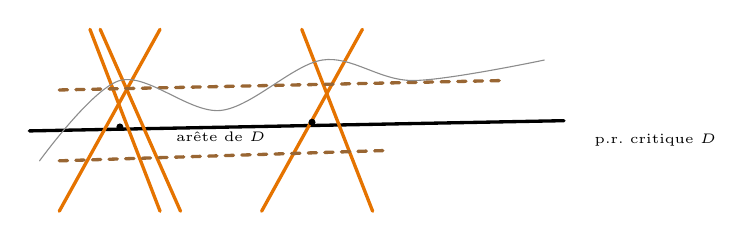
\begin{tikzpicture}[x=1mm,y=1mm,line cap=round,line join=round,font=\scriptsize]
\draw[very thick] (1.3,-16.7) -- (69.2,-15.4);
\draw[Or,very thick] (5.1,-26.9) -- (17.9,-3.8);
\draw[Or,very thick] (10.3,-3.8) -- (20.5,-26.9);
\draw[Or,very thick] (30.8,-26.9) -- (43.6,-3.8);
\draw[Or,very thick] (35.9,-3.8) -- (44.9,-26.9);
\draw[Or,very thick] (9,-3.8) -- (17.9,-26.9);
\node[pt] at (12.8,-16.2) {};
\node[pt] at (37.2,-15.6) {};
\draw[Br,dashed,very thick] (5.1,-11.5) -- (61.5,-10.3);
\draw[Br,dashed,very thick] (5.1,-20.5) -- (46.2,-19.2);
\draw[pencil] plot[smooth, tension=0.55] coordinates {(2.6,-20.5) (12.8,-10.3) (25.6,-14.1) (38.5,-7.7) (50,-10.3) (66.7,-7.7)};
\node[inner sep=1pt] at (25.6,-17.4) {\tiny arête de $D$};
\node[inner sep=1pt] at (80.8,-17.9) {\tiny p.r.\ critique $D$};
\end{tikzpicture}
\end{document}
